In this section we pursue with the analysis of data scrapped on several cryptocurrency subreddits. More precisely, we use social media analytics on the network that we built in the previous section. Firstly, we investigate if our network follows a power law distribution as it should. Secondly, we discuss the results of the pagerank algorithm on the network. Thirdly, we run Louvain community detection algorithm and compare the results with the existing subreddits.

The power law distribution in a network can be understood as ``a few users are very popular and a lot of users are mildly or not popular at all''. Intuitively, this relation holds in our network composed of vertices as users and edges representing the comment relation. Indeed, when browsing Reddit in general, we may notice that a few comments (users) are very popular (have a very high score) as others are not. This intuition reveals itself true when plotting the node degree distribution (see fig. \ref{fig:deg_dist}). This is encouraging in relation to our network model and further analysis.
\begin{figure}[Hb!]
    \centering
    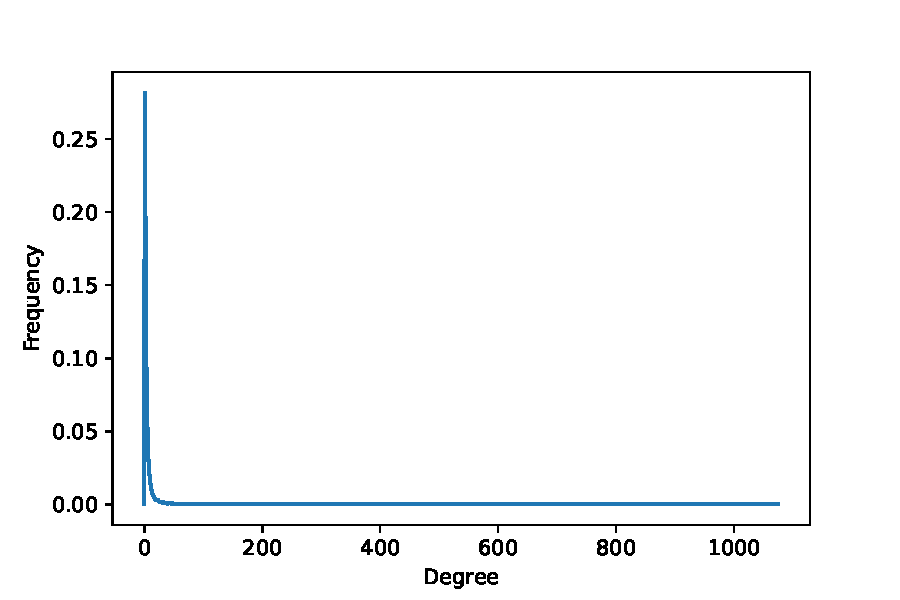
\includegraphics[width=0.3\textwidth]{figures/deg_dist.pdf}
    \caption{The network follows a power law distribution: a lot of users have few comments on their posts and a few users have a lot of comments on their posts.}
    \label{fig:deg_dist}
\end{figure}

